\documentclass[12pt letter]{report}
\input{./template/preamble}
\input{./template/macros}
\input{./template/letterfonts}

\title{\Huge{Basic Structures: Sets, Functions, Sequences, Sums, and Matrices}}
\author{\huge{Madiba Hudson-Quansah}}
\date{}
\usepackage{parskip}
\usepackage{proof}
\setcounter{tocdepth}{4}
\setcounter{secnumdepth}{4}


\begin{document}
\maketitle
\newpage
\pdfbookmark[section]{\contentsname}{too}
\tableofcontents
\pagebreak

\chapter{Sets}

\dfn{Set}{
	An unordered collection of objects, called \textit{elements} or \textit{members} of the set. A set contains elements
	and, we can denote this as  $a \in A$ where $a$ is an element of the set $A$, or $a \notin A$, where $a$ is not an
	element of the set $A$.
}

There are several ways to describe a set:
\begin{description}
	\item[Roster notation] $\left\{ 1, 2, 3, 4, 5 \right\} $
	\item [Set-Builder notation] Where all the elements of a set are described by a property they satisfy.i.e. The set $O$ of
	      all odd positive numbers less than 10 can be expressed as $ O =  \left\{ x  \mid  x \text{ is an odd positive
			      integer less than } 10  \right\}  $ or specifying the domain of discourse, $O =  \left\{ x \in \mathbb{Z}^{+}
		      \mid x \text{ is odd and } x < 10 \right\} $, or the set of all positive rational numbers $\mathbb{Q}^{+}$
	      can be expressed as $\mathbb{Q}^{+} = \left\{ x \in \mathbb{R}  \mid x = \frac{p}{q}
		      \text{, for some positive integers $q$ and $p$}\right\}  $
\end{description}

\dfn{Equality of Sets}{
	Two sets $A$ and $B$ are equal if and only if they have the same elements. Therefore, $\forall x \left( x \in A
		\leftrightarrow x \in B \right) $, We write $A = B$ if this is the case.
}

\dfn{Empty / Null Set}{
	A set with no elements, denoted by $\O$ or $ \left\{  \right\}  $. Can be expressed as $\{x \mid F \} $

}

\dfn{Singleton Set}{
	A set with exactly one element, denoted by $\left\{ a \right\} $. The set $ \left\{ \O \right\}  $ is a singleton set as
	it is a set with one element, the empty set.
}

\subsection{Set Definitions}

\subsubsection{Natural numbers}

\[
	\mathbb{N} = \left\{ 1, 2, 3, 4, 5, \ldots \right\}
\]

\subsubsection{Integers}

\[
	\mathbb{Z} = \left\{ \ldots, -3, -2, -1, 0, 1, 2, 3, \ldots \right\}
\]

\subsubsection{Positive Integers}

\[
	\mathbb{Z}^{+} = \left\{ 1, 2, 3, 4, 5, \ldots \right\}
\]

\subsubsection{Rational numbers}

\[
	\mathbb{Q} = \left\{ \frac{p}{q} \mid p, q \in \mathbb{Z} \text{ and } q \neq 0 \right\}
\]

\subsubsection{Irrational Numbers}
\[
	\mathbb{I} = \left\{ x \mid x \text{ is a number that cannot be expressed as a fraction} \right\}
\]

\subsubsection{Real numbers}

\[
	\mathbb{R} = \left\{ x \mid x \text{ is a point on the number line} \right\}
\]

Or

\[
	\mathbb{R} = \mathbb{Q} \cup \mathbb{I}
\]

\subsubsection{Positive Real numbers}
\[
	\mathbb{R}^{+} = \left\{ x \in \mathbb{R} \mid x > 0 \right\}
\]

\subsubsection{Complex numbers}

\[
	\mathbb{C} = \left\{ a + bi \mid a, b \in \mathbb{R} \text{ and } i^{2} = -1 \right\}
\]


\subsection{Venn Diagrams}

\dfn{Universal Set}{
	The set of all objects under consideration, denoted by $U$. Can be expressed as $\{x  \mid T\} $
}

Sets can be graphically represented using Venn diagrams. A Venn diagram is a collection of simple closed curves, especially
circles, that represent sets. In Venn diagrams the universal set $U$ which contains all the objects under consideration
is represented by a rectangle, and the sets are represented by circles within the rectangle, with points inside the
circles representing elements of the sets.

% Venn diagram for the set of vowels in the English language


\subsection{Subsets}

\dfn{Subset}{
	A set $A$ is a \textit{subset} of a set $B$ if and only if every element of $A$ is also an element of $B$. Denoted
	by $A \subseteq B $.
}

We see that $A \subseteq B$ if and only if
\[
	\forall x \left( x \in A \to x \in B \right)
\]

Is true. I.e. If $x \in A$, then $x \in B$. To disprove this we need to show that $\exists x \left( x \in A \wedge x
	\notin B \right) $

Shown graphically: \\

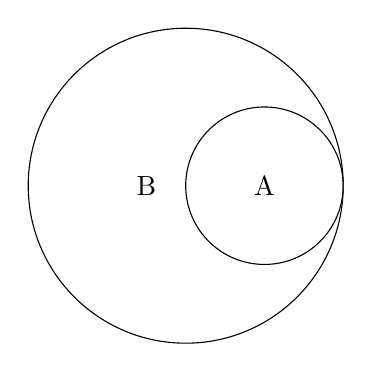
\begin{tikzpicture}
	\draw (0,0) circle (1cm);
	\draw (-1,0) circle (2cm);
	\node at (0,0) {A};
	\node at (-1.5, 0) {B};
\end{tikzpicture}

\ex{}{
	The set of integers with squares less than 100 is not a subset of the set of nonnegative integers
	because -1 is in the former set [as $\left( -1 \right) ^2 < 10$], but not the later set. The set of people who
	have taken discrete mathematics at your school is not a subset of the set of all computer science
	majors at your school if there is at least one student who has taken discrete mathematics who is
	not a computer science major.
}

\thm{}{
	For every set $S$
	\begin{enumerate}
		\item $\O \subseteq S$
		\item $S \subseteq S$
	\end{enumerate}

	\begin{enumerate}
		\item
		      \begin{myproof}
			      We will prove that $\O \subseteq S$, using a vacuous proof \\
			      Let $S$ be a set. \\
			      To show $\O \subseteq S$ we must show that $\forall x \left( x \in \O \to x \in S \right) $ is $T$. \\
			      Because $\O$ contains no elements $x \in  \O$ is always $F$ \\
			      This follows that the implication $x \in \O \to x \in S$ is always $T$ \\
			      Hence $\O \subseteq S$ \\
		      \end{myproof}
		\item
		      \begin{myproof}
			      We will prove that $S \subseteq S$, using a direct proof \\
			      Let $S$ be a set\\
			      To show $S \subseteq S$ we must show that $\forall x \left( x \in S \to x \in S \right) $ is $T$ \\
			      Assume $x \in S$ \\
			      Because $x \in S$ is always $T$, the implication $x \in S \to x \in S$ is always $T$ \\
			      $\therefore$ $\forall x \left( x \in S \to x \in S \right) $ is $T$\\
			      Hence $S \subseteq S$ \\
		      \end{myproof}

	\end{enumerate}
}

\dfn{Proper subset}{
	A set $A$ is \textit{proper subset} of a set $B$ if and only if every element of $A$ is also an element of $B$ and
	$A \neq B$. Denoted by $A \subset B$. I.e.
	\[
		\exists x \left( x \notin A \wedge x \in B \right) \wedge \forall x \left( x \in A \to x \in B \right)
	\]
	Is $T$.
}

\dfn{Further Equality}{
	Two sets $A$ and $B$ are equal if $A \subseteq B \wedge  B \subseteq A$ is $T$. I.e.
	$A = \left\{ \O, \left\{ a \right\}, \left\{ a \right\}, \left\{ b \right\}, \left\{ a, b \right\}     \right\}  $
	and $B = \left\{ x  \mid x \text{ is a subset of the set } \left\{ a,b \right\}  \right\}  $ are equal.
}

\subsection{Cardinality}

\dfn{Cardinality}{
	The number of distinct elements $n$ in a set $A$. Denoted by $\left| A \right| = n$.
	Where $n$ is a non-negative integer, we say that $A$ is a finite set.
}

\dfn{Infinite set}{
	A set $A$ is infinite if it is not finite. I.e. $\left| A \right| = \infty$
}


\subsection{Power Set}

\dfn{Power Set}{
	A set containing all the subsets of a given set $A$. Denoted by $\mathcal{P} \left( A \right) $. If a set has $n$
	distinct elements, then the cardinality of the power set is $2^{n}$.
}

\ex{}{
	\qs{}{
		What is the power set of the set $ \left\{ 0,1,2 \right\}  $
	}

	\sol{
		\[
			\mathcal{P}(\left\{ 0,1,2 \right\} ) = \left\{ \O, \left\{ 0 \right\}, \left\{ 1 \right\}, \left\{ 2 \right\},,
			\left\{ 0,1 \right\}, \left\{ 0, 2  \right\}, \left\{ 1,2 \right\}, \left\{ 0,1,2 \right\}        \right\}
		\]
	}
}

\ex{}{
	\qs{}{
		What is the power set of $\O$
	}

	\sol{
		\[
			\mathcal{P}(\O) = \left\{ \O \right\}
		\]
	}

	\qs{}{
		What is the power set of $\left\{ \O \right\} $
	}

	\sol{
		\[
			\mathcal{P}\left( \left\{ \O \right\}  \right) = \left\{ \O, \left\{ \O \right\}  \right\}
		\]
	}
}

\subsection{N-Tuples}
\dfn{Ordered N-Tuple}{
	N-tuple $\left( a_1, a_2, \ldots, a_n \right) $ is the ordered collection that has $a_1$ as its first element,
	$a_2$ as its second element, \ldots, and $a_n$ as its $n$th element.
}

Two n-tuples are equal if an only if each corresponding pair of their elements is equal, i.e. $\left( a_1, a_2, \ldots,
	a_n\right) = \left( b_1, b_2, \ldots, b_n \right)  $ are equal if and only if $a_i = b_i$, for $i = 1, 2,\ldots,n$.
\\

Ordered 2-tuples are called \textit{ordered pairs}. The ordered pairs, $\left( a, b \right) $ and $\left( c, d \right) $
are equal if and only if $a = c$ and $b = d$.


\subsection{Cartesian Products}

\dfn{Cartesian Product}{
	Let $A$ and $B$ be sets. The \textit{Cartesian Product} of $A$ and $B$, denoted by $A \times B$, is the set of all
	ordered pairs $\left( a, b \right) $, where $a \in A$ and $b \in B$. I.e.
	\[
		A \times B = \left\{ \left( a, b \right)  \mid a \in A \wedge b \in  B  \right\}
	\]
	The number of items in the Cartesian product of two sets is the product of the cardinality of each set.
}

\ex{}{
	\qs{}{
		What is the Cartesian product of $A = \left\{ 1, 2 \right\} $ and $B = \left\{ a, b, c \right\} $
	}

	\sol{
		\[
			A \times B = \left\{ \left( 1,a \right), \left( 1,b \right), \left( 1,c \right), \left( 2,a  \right),
			\left( 2,b \right), \left( 2, c \right)       \right\}
		\]
	}

	\qs{}{
		Show that the Cartesian product $B \times  A$ is not equal to the Cartesian product $A \times  B$.
	}

	\sol{
		\[
			B \times A = \left\{ \left( a, 1 \right) \left( a, 2 \right), \left( b, 1 \right), \left( b,2 \right), \left(
			c,1 \right), \left( c, 2 \right)       \right\}
		\]
		$\therefore A \times B \neq B \times A$
	}

}

\dfn{Cartesian Product of more than two sets}{
	The Cartesian product of the sets $A_1,A_2,\ldots,A_n$,denoted by $A_1 \times A_2 \times \ldots \times  A_n $,
	is the set of ordered $n$-tuples $\left( a_1,a_2, \ldots,a_n \right) $, where $a_i$ belongs to $A_i$ for $i =
		1,2,\ldots, n$. I.e.
	\[
		A_1\times A_2 \times \ldots \times A_n = \left\{ \left( a_1,a_2,\ldots a_n \right)  \mid a_i \in A_i \text{ for
		}  i = 1,2,\ldots,n  \right\}
	\]
}


\ex{}{
	\qs{}{
		What is the Cartesian product $A \times  B \times C$, where $A = \left\{ 0, 1 \right\} $, $B = \left\{ 1,2 \right\}
		$, $C = \left\{ 0,1,2 \right\} $.
	}

	\sol{
		\[
			A \times B \times C = \left\{ \left( 0,1,0 \right), \left( 0,1,1 \right), \left( 0,1,2 \right), \left( 0,2,0
			\right),  \left( 0,2,1 \right), \left( 0,2,2 \right), \left( 1,1,0 \right), \left( 1,1,1 \right) ,
			\left( 1,1,2\right),   \left( 1,2,0 \right), \left( 1,2,1 \right), \left( 1,2,2 \right)
			\right\}
		\]
	}
}

We use the notation $A^2$ to denote $A \times A$, the Cartesian product of $A$ and itself. Therefore
\[
	A^n = \left\{ \left( a_1, a_2,\ldots,a_n \right)  \mid a_i \in A \text{ for } i = 1,2,\ldots,n  \right\}
\]

\ex{}{
	Suppose $A = \left\{ 1,2 \right\} $. \\
	It follows $A^2 = \left\{ \left( 1,1 \right), \left( 1,2 \right), \left( 2,1
		\right), \left( 2,2 \right)     \right\} $, \\
	and $A^3 = \left\{ \left( 1,1,1 \right), \left( 1,1,2 \right),
		\left( 1,2,1 \right), \left( 1,2,2 \right), \left( 2,1,1 \right), \left( 2,1,2 \right), \left( 2,2,1 \right), \left(
		2,2,2\right)         \right\} $
}

\ex{}{
	\qs{}{
		What are the ordered pairs in the less than or equal to relation, which contains, $\left( a, b \right) $ if $a \leq
			b$, on the set $\left\{ 0,1,2,3 \right\} $
	}

	\sol{
		Let $R$ be the relation on the set $\left\{ 0,1,2,3  \right\} $, if $a \leq b$. \\
		\begin{align*}
			R = \left\{ \left( 0,0 \right), \left( 1,1 \right), \left( 2,2 \right), \left( 3,3 \right), \left( 0,1
			\right),  \left( 0,2 \right), \left( 0,3 \right), \left( 1,2 \right), \left( 1,3 \right), \left( 2,3 \right)            \right\}
		\end{align*}
	}
}

\subsection{Set Notation with Quantifiers}


We can restrict the domain of a quantifier to a set, I.e. Where $S$ is a set $\forall x \in S \left( P \left( x \right)
	\right) $, denotes the universal quantification of $P \left( x \right) $ for all elements in the set $S$. Which is
shorthand for $\forall x \left( x \in S \to P \left( x \right)  \right) $


\ex{}{
	$\forall x \in \mathbb{R} \left( x^2 \geq 0 \right) $ means "the square of any real number is greater than or equal
	to $0$". \\
	$\exists x \in \mathbb{Z} \left( x^2 = 1 \right) $ means "there exists an integer whose square is $1$"
}

\subsection{Truth Sets and Quantifiers}

\dfn{Truth Set}{
	For a predicate $P$ the truth set of $P$ is the set of all elements in the domain of discourse that make $P$ true.
	I.e. let $S$ be a set. The truth set of $P \left( x \right) $ is
	\[
		\left\{ x \in S  \mid  P \left( x \right)  \right\}
	\]
}

\ex{}{
	\qs{}{
		What are the truth set of the predicates $P \left( x \right) $, $Q \left( x \right) $, and $R \left( x \right)
		$, where the domain is the set of integers, and $P \left( x \right)\text{: }  | x | = 1 $, $Q \left( x
			\right)\text{: }
			x^2 = 2$, and $R \left( x \right)\text{: }  | x | = x  $
	}

	\sol{

		\noindent The truth set of $P$ is $\left\{ x \in \mathbb{Z}  \mid  |x| = 1 \right\} $ \\
		The truth set of $Q$ is $\left\{ x \in Z  \mid x^2 = 2 \right\} $ \\
		The truth set of $R$ is $\left\{ x \in \mathbb{Z}  \mid  |x| = x \right\} $
	}
}

\nt {
	$\forall x P \left( x \right) $ is $T$ over the domain $U$ if and only if the truth set of $P$ is $U$.
	\\
	$\exists x P \left( x \right) $ is $T$ over the domain $U$ if and only if the truth set of $P$ is not empty.
}

\section{Exercises}

\qs{}{
	List the members of these sets
	\begin{enumerate}
		\item $\left\{ x  \mid x \text{ is the square of an integer and } x < 100 \right\} $
		\item $\left\{ x  \mid x \text{ is an integer such that } x^2 = 2 \right\} $
	\end{enumerate}
}

\sol{
	\begin{enumerate}
		\item $\left\{ 1, 4, 9, 16, 25, 36, 49, 64, 81 \right\} $
		\item $\O$
	\end{enumerate}
}

\qs{}{
	Use set builder notation to describe the following sets
	\begin{enumerate}
		\item $\left\{ -3,-2,-1,0,1,2,3 \right\} $
		\item $\left\{ m,n,o,p \right\} $
	\end{enumerate}
}

\sol{
	\begin{enumerate}
		\item $\left\{ x  \mid -3 \leq x \leq 3  \right\} $
		\item $\left\{ x  \mid x \text{ is a letter in the word monopoly excluding "l" and "y" } \right\} $
	\end{enumerate}
}

\qs{}{
	Suppose that $A = \left\{ 2, 4, 6 \right\} $, $B = \left\{ 2, 6 \right\} $, $C = \left\{ 4, 6 \right\} $ and $D =
		\left\{ 4,6,8 \right\} $. Determine which of these sets are subsets of which other sets.
}

\sol{
	\begin{align*}
		B \subseteq  A \\
		C \subseteq A  \\
		C \subseteq D  \\
	\end{align*}
}

\qs{}{
	Suppose that $A$, $B$, $C$, are sets such that $A \subseteq B$ and $B \subseteq C$. Show that $A \subseteq C$
}

\sol{

	\begin{align*}
		A \subseteq B  \text{ means } \forall x \left( x \in A \to x \in  B \right) \\
		B \subseteq C \text{ means } \forall x \left( x \in B \to x \in C \right)   \\
		A \subseteq C \text{ means } \forall x \left( x \in A \to x \in  C \right)  \\
	\end{align*}

	\begin{align*}
		\begin{deduction}
			\premise{ \forall x \left( x \in  A \to x \in  B \right)  }
			\premise{ \forall x \left( x \in  B \to x \in C \right) }
			\conclusion{ \forall x \left( x \in A \to x \in C \right) }
		\end{deduction}
	\end{align*}

	\gdef\rownumber{\stepcounter{magicrownumbers}\arabic{magicrownumbers}}
	\begin{table}[h!]
		\begin{center}
			\begin{tabular}{ | @{\makebox[3em][r]{\rownumber\space}} | c | c | }
				\hline
				\multicolumn{1}{ | @{\makebox[3em][r]{~}} |c| }{Steps} & \multicolumn{1}{|c|}{Reasons}        \\
				\hline
				\hline
				$ \forall x \left( x \in  A \to x \in  B \right)  $    & Premise 1                            \\
				$ \forall x \left( x \in  B \to x \in C \right) $      & Premise 2                            \\
				$x \in  A \to x \in  B$                                & Universal Instantiation of 1         \\
				$x \in B \to x \in C$                                  & Universal Instantiation of 2         \\
				$x \in A \to x \in C$                                  & By Hypothetical Syllogism of 3 and 4 \\
				$\forall x \left( x \in A \to x \in C \right) $        & Universal generalization of 5        \\
				\hline
			\end{tabular}
		\end{center}
	\end{table}
}

\qs{}{
	Find the power set of each of these sets, where $a$ and $b$ are distinct elements.
	\begin{enumerate}
		\item $\{a\} $
		\item $\{a, b\} $
		\item $\{\O, \{\O\} \} $
	\end{enumerate}
}

\sol{
	\begin{enumerate}
		\item $\mathcal{P}\left( \{a\}  \right)  = \{\O, \{a\} \} $
		\item $\mathcal{P}(\{a,b\} ) = \{\O, \{a\}, \{b\}, \{a,b\}   \} $
		\item $\mathcal{P}(\{\O, \{\O\} \} ) = \{\O, \{\O\}\, \{\{\O\} \}, \{\O, \{\O\} \}   \} $
	\end{enumerate}
}


\chapter{Set Operations}

\section{Set Operations}

\subsection{Union}

\dfn{Union}{
	Let $A$ and $B$ be sets. The \textit{union} of $A$ and $B$, denoted by $A \cup B$, is the set of all elements that
	are either in $A$ or in $B$ or in both. I.e.
	\[
		A \cup B = \left\{ x  \mid  x \in A \vee x \in B \right\}
	\]
}

\subsection{Intersection}

\dfn{Intersection}{
	Let $A$ and $B$ be sets. The \textit{intersection} of $A$ and $B$, denoted by $A \cap B$, is the set of all elements
	that are in both $A$ and $B$. I.e.
	\[
		A \cap B = \left\{ x  \mid  x \in A \wedge x \in B \right\}
	\]
}

\subsection{Complement}

\dfn{Complement}{
	Let $A$ be a set. The \textit{complement} of the set A (with respect to $U$), denoted by $\overline{A}$ is the set
	$U - A$. I.e.
	\[
		\overline{A} = \left\{ x \in U  \mid x \notin A \right\}
	\]
}

\subsection{Difference}

\dfn{Difference}{
	Let $A$ and $B$ be sets.  The \textit{difference} of $A$ and $B$, denoted by $A - B$, is the set of all elements
	that are in $A$ but not in $B$. I.e.
	\[
		A - B = \left\{ x  \mid  x \in A \wedge x \notin B \right\}
	\]
	Or
	\[
		A - B = A \cap \overline{B}
	\]
}

\subsection{Symmetric Difference}

\dfn{Symmetric Difference}{
	Let $A$ and $B$ be sets. The \textit{symmetric difference} of $A$ and $B$, denoted by $A \oplus  B$, is the set
	of all elements that are in exactly one of $A$ and $B$. I.e.
	\[
		A \oplus B = \left( A - B \right) \cup \left( B - A\right)
	\]
}

\ex{}{
	\qs{}{
		\begin{align*}
			U = \left\{ 0,1,2,3,4,5,6,7,8,9,10 \right\} \\
			A = \left\{ 1,2,3,4,5 \right\}              \\
			B = \left( 4,5,6,7,8 \right)
		\end{align*}
		What is $A \oplus B$
	}

	\sol{
		\[
			A \oplus B = \left\{ 1,2,3,6,7,8 \right\}
		\]
	}
}

\subsection{The Cardinality of the Union of Two Sets}

The cardinality of the union of two sets $A$ and $B$ is given by
\[
	\left| A \cup B \right| = \left| A \right| + \left| B \right| - \left| A \cap B \right|
\]

\section{Set Identities}

\subsection{Identity Laws}

\begin{align*}
	A \cap   U = A \\
	A \cup  \O = A
\end{align*}

\subsection{Domination Laws}

\begin{align*}
	A \cup U = U \\
	A \cap \O = \O
\end{align*}

\subsection{Idempotent Laws}

\begin{align*}
	A \cup A = A \\
	A \cap A = A
\end{align*}

\subsection{Complementation Law}
\[
	\overline{\left( \overline{A} \right) } = A
\]

\subsection{Commutative Laws}

\begin{align*}
	A \cup B = B \cup A \\
	A \cap B = B \cap A
\end{align*}

\subsection{Associative Laws}

\begin{align*}
	A \cup \left( B \cup  C \right)  = \left( A \cup B \right)  \cup C \\
	A \cap \left( B \cap C  \right)  = \left( A \cap B \right)  \cap C
\end{align*}

\subsection{Distributive Laws}

\begin{align*}
	A \cup \left( B \cap C \right)  = \left( A \cup B \right)  \cap \left( A \cup C \right) \\
	A \cap \left( B \cup C  \right)  = \left( A \cap B \right)  \cup \left( A \cap C \right)
\end{align*}

\subsection{De Morgan's Laws}
\begin{align*}
	\overline{A \cap  B} = \overline{A} \cup \overline{B} \\
	\overline{A \cup B } = \overline{A} \cap \overline{B}
\end{align*}

\subsection{Absorption Laws}
\begin{align*}
	A \cup \left( A \cap B \right) = A \\
	A \cap  \left( A \cup B  \right)  = A
\end{align*}

\subsection{Complement Laws}
\begin{align*}
	A \cup \overline{A} = U \\
	A \cap \overline{A} = \O
\end{align*}

\subsection{Proving Set Identities}

There are different ways to prove set identities, these include:
\begin{itemize}
	\item Proving each set is a subset of the other
	\item Using set builder notation and propositional logic
	\item Using Membership tables
\end{itemize}

\dfn{Membership Table}{
	A table that shows the truth value of a predicate for all possible combinations of truth values of its variables.
}


\ex{}{
	\qs{}{
		Prove that
		\[
			\overline{A \cap B} = \overline{A} \cup \overline{B}
		\]
	}

	\noindent Using propositional logic:
	\begin{myproof}
		We prove this identity by showing that each set is a subset of the other. I.e.\\
		\[
			\overline{A \cap  B} \subseteq \overline{A} \cup  \overline{B} \wedge \overline{A} \cap \overline{B} \subseteq
			\overline{A \cap B}
		\]
		\begin{align*}
			\overline{A \cap B} \subseteq \overline{A} \cup \overline{B} \text{ means } \forall x \left( x \in
			\overline{A \cap B} \to x \in \overline{A} \cup  \overline{B} \right) \\
			\overline{A} \cup \overline{B} \subseteq \overline{A \cap B} \text{ means } \forall x \left( x \in
			\overline{A} \cup \overline{B} \to x \in \overline{A \cap B} \right)  \\
		\end{align*}
		Assume that $x \in  \overline{A \cap  B}$\\
		\begin{align*}
			x \in  \overline{A \cap B}                               \tag*{Assumption}            \\
			x \notin A \cap B                                     \tag*{Definition of Complement} \\
			\neg \left( x \in A \cap B \right)                    \tag*{Definition of $\notin$ }  \\
			\neg \left( x \in A \wedge x \in B \right)   \tag*{Definition of intersection}        \\
			\neg \left( x \in A \right) \vee \neg \left( x \in  B  \right) \tag*{ By First De Moragn's Law for propositional
			logic}                                                                                \\
			x \notin A \vee x \notin B \tag*{Definition of Complement}                            \\
			x \in \overline{A} \cup \overline{B} \tag*{Definition of union}
		\end{align*}
		Then we assume $x \in \overline{A} \cup \overline{B}$
		\begin{align*}
			x \in \overline{A} \cup \overline{B} \tag*{Assumption}                                               \\
			x \notin A \vee x \notin B \tag*{Definition of union}                                                \\
			\neg \left( x \in A \right)  \vee  \neg \left( x \in B \right)  \tag*{Definition of Complement}      \\
			\neg \left( x \in A \wedge  x \in B \right) \tag*{By Second De Morgan's Law for propositional logic} \\
			x \notin A \wedge x \notin B \tag*{Definition of Complement}                                         \\
			x \notin A \cap B \tag*{Definition of intersection}                                                  \\
			x \in \overline{A \cap B} \tag*{Definition of Complement}
		\end{align*}

	\end{myproof}
	\noindent Using set builder notation
	\begin{align*}
		\overline{A \cap B} & = \{ x  \mid x \notin A \cap B\} \tag*{Definition of Complement}                                                \\
		                    & = \{x  \mid \neg \left( x \in \left( A \cap B \right)  \right) \} \tag*{Definition of $\notin$}                 \\
		                    & = \{x  \mid \neg \left( x \in A \wedge x \in B \right) \} \tag*{Definition of Intersection}                     \\
		                    & = \{x  \mid \neg \left( x \in A \right) \vee \neg \left( x \in B \right)  \} \tag*{By First De Morgan's Law for
		propositional logic}                                                                                                                  \\
		                    & = \{x  \mid x \notin A \vee x \notin B\} \tag*{Definition of Complement}                                        \\
		                    & = \{x | x \in \overline{A} \cup \overline{B}\} \tag*{Definition of union}                                       \\
		                    & = \overline{A} \cup \overline{B}                                                                                \\
	\end{align*}
}

\section{Generalized Unions and Intersections}

\dfn{Generalized Union}{
	The union of a collection of sets  that contains those elements that are members of at least one set in the
	collection. Denoted by
	\[
		A_1 \cup A_2 \cup \ldots \cup A_n = \bigcup_{i = 1} ^n A_i
	\]
	Where $A_1 \cup A_2 \cup  \ldots A_n$ is the union of sets $A_1,A_2,\ldots,A_n$
}

\dfn{Generalized Intersection}{
	The intersection of a collection of sets that contains those elements that are members of all the sets in the
	collection. Denoted by
	\[
		A_1 \cap A_2 \cap \ldots A_n = \bigcap_{i = 1} ^n A_i
	\]
	Where $A_1 \cap A_2 \cap \ldots \cap A_n$ is the intersection of sets $A_1,A_2,\ldots,A_n$
}

\ex{}{
	For $i = 1,2,\ldots,$ let $A_i = \{i,i+1,i+2,\ldots\} $. Then.
	\[
		\bigcup_{i = 1} ^n A_i = \bigcup_{i = 1} ^n \{i, i+1, i+2,\ldots\} = \{1,2,3,\ldots\}
	\]
	and
	\[
		\bigcap_{i = 1} ^{n}A_i = \bigcap_{i = 1} ^{n}\{i,i+1,i+2,\ldots\} = \{n, n+1, n+2\} = A_n
	\]
}

We can extend this notation to other families of sets I.e.
\[
	A_1 \cup A_2 \cup \ldots \cup A_n \cup \ldots = \bigcup_{i = 1} ^{\infty}A_i
\]
Denotes the union of the sets $A_1,A_2,\ldots,A_n,\ldots$, and the intersection of these sets is denoted by
\[
	A_1 \cap A_2 \cap \ldots \cap A_n \cap \ldots = \bigcap_{i = 1} ^{\infty}A_i
\]

Generally when $I$ is set, the notations $\bigcap_{i \in  I}A_i $ and $\bigcup_{i \in  I}A_i $ are used to denote the
intersection and union of the sets $A_i$ for $i \in I$, respectively, where
\[
	\bigcap_{i \in  I} A_i = \{x  \mid \forall i \in I \left( x \in A_i \right) \}
\]
and
\[
	\bigcup_{i \in  I}  A_i = \{x  \mid \exists i \in I \left( x \in A_i \right) \}
\]

\ex{}{
	Suppose $A_i = \{1,2,3,\ldots,i\} $ for $i = \{1,2,3,\ldots\} $ Then
	\[
		\bigcup_{i = 1} ^{\infty} A_i = \bigcup_{i = 1}^{\infty}  \{1,2,3,\ldots,i\}  = \mathbb{Z}^{+}
	\]

	and
	\[
		\bigcap_{i = 1} ^{\infty}A_i = \bigcap_{i = 1} ^{\infty} \{1,2,3,\ldots,i\}  = \{1\}
	\]
}

\section{Computer Representation Of Sets}

Assume that the universal set $U$ is finite. First, specify an arbitrary ordering of the elements of $U$, e.g. $a_1, a_2,
	a_3, \ldots,a_n$. Represent subset $A$ of $U$ with the bit string of length $n$, where the $i$th bit in this string is
$1$ if $a_i$ belongs to $A$ and is $0$ if $a_i$ does not belong to $A$.

\ex{}{
	\qs{}{
		Let $U = \{1,2,3,4,5,6,7,8,9,10\} $ and the ordering of the elements of $U$ has the elements in increasing order,
		i.e. $a_i = i$. What bit strings represent the subset of all odd integers in $U$, the subset of all even integers in
		$U$, and the subset of all integers not exceeding $5$ in $U$.
	}

	\sol{
		Odd integers - $1010101010$\\
		Even integers - $0101010101$\\
		Less than or equal to $5$ - $1111100000$

	}
}

To find the bit strings that represent the union, intersection, and complement of two sets, we can use the bitwise OR,
bitwise AND, and bitwise NOT operations, respectively.

\ex{}{
	\qs{}{
		The bit strings for the sets $\{1,2,3,4,5\} $ and $\{1,3,5,7,9\} $ are $1111100000$ and $1010101010$ respectively.
		Find the union and intersection of these sets.
	}

	\sol{

		\begin{align*}
			\vee \quad
			\begin{split}
				11\,1110\,0000 \\
				10\,1010\,1010 \\
				\hline
				11\,1110\,1010 \\
			\end{split}
		\end{align*}

		\begin{align*}
			\wedge \quad
			\begin{split}
				11\,1110\,0000 \\
				10\,1010\,1010 \\
				\hline
				10\,1010\,0000 \\
			\end{split}
		\end{align*}

	}
}

\section{Exercises}

\qs{}{
	List the members of these sets
	\begin{enumerate}
		\item  $\left\{ x  \mid x \text{ is a real number such that } x^2 = 1 \right\}$
		\item $\{x | x \text{ is a positive integer less than 12}\} $
		\item $\{x | x \text{ is the square of an integer and } x < 100\} $
		\item $ \left\{ x  \mid  x \text{ is an integer such that } x^2 = 2 \right\} $
	\end{enumerate}
}

\sol{
	\begin{enumerate}
		\item $\left\{ -1, 1 \right\} $
		\item $\{1,2,3,4,5,6,7,8,9,10,11\} $
		\item $\{0, 1, 4, 9, 16, 25, 36, 49, 64, 81\} $
		\item $ \O $
	\end{enumerate}
}

\qs{}{
	Use set builder notation to show that:
	\begin{enumerate}
		\item $A \cup U = U$
		\item $A \cap \O = \O$
		\item $A \cup  \overline{A} = U$
		\item $A \cap \overline{A} = \O$
	\end{enumerate}
}

\sol{
	\begin{enumerate}
		\item
		      \begin{align*}
			      A \cup U & = \{ x  \mid x \in A \cup U\} \tag*{Set builder notation}               \\
			               & = \{x  \mid x \in A \vee   x \in U \} \tag*{Definition of Union}        \\
			               & = \{x  \mid  x \in A \vee  T\} \tag*{Definition of Universal Set}       \\
			               & = \{x  \mid T \} \tag*{By First Domination law for propositional logic} \\
			               & = U \tag*{Definition of Universal Set}                                  \\
		      \end{align*}
		\item
		      \begin{align*}
			      A \cap \O & = \{ x \mid x \in A \cap \O\}  \tag*{Set builder notation}               \\
			                & = \{x  \mid x \in A \wedge x \in \O \} \tag*{Definition of Intersection} \\
			                & = \{x  \mid x \in A \wedge  F\} \tag*{Definition of Empty set}           \\
			                & = \{x  \mid F\} \tag*{By Second Domination Law for propositional logic}  \\
			                & = \O \tag*{Definition of Empty set}                                      \\
		      \end{align*}
		\item
		      \begin{align*}
			      A \cup \overline{A} & = \{x  \mid x \in A \cap \overline{A}\}  \tag*{Set builder notation}                       \\
			                          & = \{x  \mid x \in A \vee  x \in \overline{A}\} \tag*{Definition of Union}                  \\
			                          & = \{x  \mid x \in A \vee  x \notin A\} \tag*{Definition of Complement}                     \\
			                          & = \{x  \mid x  \in A \vee  \neg \left( x \in A \right)  \} \tag*{Definition of Complement} \\
			                          & = \{x  \mid T\} \tag*{By First Negation Law for propositional logic}                       \\
			                          & = U \tag*{Definition of Universal set}                                                     \\
		      \end{align*}
		\item
		      \begin{align*}
			      A \cap \overline{A} & = \{ x  \mid x \in A \cap \overline{A}\} \tag*{Set builder notation}                     \\
			                          & = \{x  \mid x \in A \wedge x \in \overline{A} \} \tag*{Definition of intersection}       \\
			                          & = \{x  \mid x \in A \wedge \left( x \notin A \right)  \} \tag*{Definition of Complement} \\
			                          & = \{x | x \in A \wedge  \neg \left( x \in  A \right) \} \tag*{Definition of
			      Complement}                                                                                                    \\
			                          & = \{x  \mid F\} \tag*{By Second Negation law of propositional logic}                     \\
			                          & = \O \tag*{Definition of $\O$}                                                           \\
		      \end{align*}
	\end{enumerate}
}

\qs{}{
	Let $A$ and $B$ be sets. Show that
	\begin{enumerate}
		\item $\left( A \cap B \right) \subseteq A $
		\item $A \subseteq \left( A \cup B \right) $
		\item $A - B \subseteq A$
		\item $A \cap \left( B - A \right) = \O $
		\item $A \cup \left( B - A \right) = A \cup B $
	\end{enumerate}
}

\sol{
	\begin{enumerate}
		\item
		      \begin{align*}
			      \left( A \cap B \right) \subseteq A \text{ means } \forall x \left( x \in \left( A \cap B \right) \to x \in A  \right)
		      \end{align*}
		      Assume $x \in \left( A \cap B \right) $
		      \gdef\rownumber{\stepcounter{magicrownumbers}\arabic{magicrownumbers}}
		      \begin{table}[h!]
			      \begin{center}
				      \begin{tabular}{ | @{\makebox[3em][r]{\rownumber\space}} | c | c | }
					      \hline
					      \multicolumn{1}{ | @{\makebox[3em][r]{~}} |c| }{Steps} & \multicolumn{1}{|c|}{Reasons} \\
					      \hline
					      \hline
					      $x \in A \cap B$                                       & Assumption                    \\
					      $x \in A \wedge x \in B$                               & Definition of intersection    \\
					      $x \in A$                                              & Simplification of 2           \\
					      \hline
				      \end{tabular}
			      \end{center}
		      \end{table}
		      \\
		      $\therefore$ $x \in \left( A \cap B \right) \to x \in A $\\
		      Conclusion: $\left( A \cap B \right) \subseteq A $
		\item
		      \begin{myproof}
			      \[
				      A \subseteq \left( A \cup B \right)  \text{ means } \forall x \left( x \in A \to x \in A \cup B \right)
			      \]
			      \gdef\rownumber{\stepcounter{magicrownumbers}\arabic{magicrownumbers}}
			      \begin{table}[h!]
				      \begin{center}
					      \begin{tabular}{ | @{\makebox[3em][r]{\rownumber\space}} | c | c | }
						      \hline
						      \multicolumn{1}{ | @{\makebox[3em][r]{~}} |c| }{Steps} & \multicolumn{1}{|c|}{Reasons} \\
						      \hline
						      \hline
						      $x \in A$                                              & Premise                       \\
						      $x \in A \wedge x \in B$                               & Addition                      \\
						      $x \in A \cup B $                                      & Definition of Union           \\
						      \hline
					      \end{tabular}
				      \end{center}
			      \end{table}\\
			      $\therefore$ $x \in A \to x \in A \cup B$\\
			      Conclusion: $A \subseteq A \cup B$
		      \end{myproof}

		\item
		      \begin{myproof}
			      $A - B \subseteq A$ means $\forall x \left( x \in A - B \to x \in  A \right) $ \\
			      Assume $ x \in A - B$\\
			      \gdef\rownumber{\stepcounter{magicrownumbers}\arabic{magicrownumbers}}
			      \begin{table}[h!]
				      \begin{center}
					      \begin{tabular}{ | @{\makebox[3em][r]{\rownumber\space}} | c | c | }
						      \hline
						      \multicolumn{1}{ | @{\makebox[3em][r]{~}} |c| }{Steps} & \multicolumn{1}{|c|}{Reasons} \\
						      \hline
						      \hline
						      $x \in A - B$                                          & Assumption                    \\
						      $x \in A \wedge x \notin B$                            & Definition of Difference      \\
						      $x \in A$                                              & By Simplification on 2        \\
						      \hline
					      \end{tabular}
				      \end{center}
			      \end{table}\\
			      $\therefore$ $x \in A - B \to x \in A$ \\
			      Hence $A - B \subseteq A$
		      \end{myproof}

		\item
		      \begin{align*}
			      A \cap \left( B - A \right) & =  A \cap \left( B \cap \overline{A} \right) \tag*{Definition of Difference} \\
			                                  & = B \cap \left( A \cap \overline{A} \right) \tag*{By Second Associative Law} \\
			                                  & = B \cap \O \tag*{By Second Complement Law}                                  \\
			                                  & = \O \tag*{By Second Domination Law}                                         \\
		      \end{align*}
		      Hence $A \cap \left( B - A \right) = \O $

		\item
		      \begin{align*}
			      A \cup \left( B - A \right) & = A \cup \left( B \cap \overline{A} \right)  \tag*{Definition of Difference}                       \\
			                                  & = \left( A \cup B \right) \cap \left( A \cup \overline{A} \right) \tag*{By First Distributive Law} \\
			                                  & = \left( A \cup B \right) \cap U  \tag*{By First Complement Law}                                   \\
			                                  & = \left( A \cap U \right) \cup \left( B \cap U  \right) \tag*{By Second
			      Distributive Law}                                                                                                                \\
			                                  & = A \cup B \tag*{By First Identity Law}                                                            \\
		      \end{align*}
		      Hence $A \cup \left( B - A \right) = A \cup B $

	\end{enumerate}
}

\qs{}{
	Show that if $A$ is a subset of a universal set $U$, then
	\begin{enumerate}
		\item $A \oplus A = \O$
		\item $A \oplus  \O = A$
		\item $A \oplus U = \overline{A}$
		\item $A \oplus \overline{A} = U$
	\end{enumerate}
}

\sol{
	\begin{enumerate}
		\item
		      \begin{align*}
			      A \oplus A & = \{x  \mid A \oplus A\} \tag*{Set Builder Notation}                                                   \\
			                 & = \{x  \mid x \in \left( A - A \right) \cup \left( A - A \right)  \} \tag*{Definition of Symmetric
			      Difference}                                                                                                         \\
			                 & = \{x  \mid \left( x \in A - A \right) \vee \left( x \in A - A \right)   \} \tag*{Definition of Union} \\
			                 & = \{x  \mid x \in A - A\} \tag*{By Idempotent Law for propositional logic}                             \\
			                 & =  \{ x  \mid \left( x \in A \right) \wedge \left( x \notin A \right)   \}
			      \tag*{Definition of Difference}                                                                                     \\
			                 & = \{x  \mid \left( x \in A \right) \wedge \neg \left( x \in A \right)  \}
			      \tag*{Definition of Complement}                                                                                     \\
			                 & = \{x  \mid F\} \tag*{By First Negation Law for propositional logic }                                  \\
			                 & = \O                                                                                                   \\
		      \end{align*}
		      Hence $A \oplus A = \O$
		\item
		      \begin{align*}
			      A \oplus \O & = \{ x  \mid A \oplus \O\} \tag*{Set Builder Notation}                                               \\
			                  & = \{x  \mid x \in \left( A - \O \right) \cup \left( \O - A \right)  \} \tag*{Definition of Symmetric
			      Difference}                                                                                                        \\
			                  & = \{x  \mid x \in \left( A - \O \right) \vee  x \in \left( \O - A \right)  \} \tag*{Definition of
			      Union}                                                                                                             \\
			                  & = \{x  \mid \left( x \in A \wedge  x \notin \O \right)\vee  \left( x \in \O \wedge x \notin A
			      \right)   \} \tag*{Definition of Difference}                                                                       \\
			                  & = \{x  \mid \left( x \in A \wedge  \neg \left( x \in \O \right)  \right) \vee  \left( x
			      \in \O \wedge
			      \neg  \left( x \in A \right) \right)  \} \tag*{Definition of Complement}                                           \\
			                  & = \{x  \mid \left( x \in A \wedge  \neg \left( F \right)  \right) \vee \left( F \wedge \neg \left( x
			      \in A\right)   \right)   \} \tag*{Definition of $\in $}                                                            \\
			                  & = \{x  \mid \left( x \in A \wedge T \right) \vee \left( F \right)  \} \tag*{By Second Domination Law
			      for propositional logic}                                                                                           \\
			                  & = \{x \mid x \in A \vee F\} \tag*{By First Identity Law for propositional logic}                     \\
			                  & = \{x  \mid x \in A\} \tag*{By Second Identity Law for propositional logic}                          \\
			                  & = A \tag*{Definition of set $A$}                                                                     \\
		      \end{align*}
		      By set identities:
		      \begin{align*}
			      A \oplus \O & = \left( A - \O \right)  \cup \left( \O - A \right)  \tag*{Definition of Symmetric Difference}       \\
			                  & = \left( A \cap \overline{\O} \right) \cup \left( \O \cap \overline{A} \right) \tag*{Definition of
			      Difference}                                                                                                        \\
			                  & = \left( A \cap U \right) \cup \left( \O \cap \overline{A} \right) \tag*{Complementation of an Empty
			      set}                                                                                                               \\
			                  & = \left( A \right) \cup \left( \O \cap \overline{A} \right) \tag*{By First Identity Law}             \\
			                  & = A \cup \left( \overline{A} \cap \O \right) \tag*{By Second Commutative Law}                        \\
			                  & = A \cup \O \tag*{By Second Domination Law}                                                          \\
			                  & = A \tag*{By Second Identity Law}                                                                    \\
		      \end{align*}
		      Hence $A \oplus \O = A$
		\item
		      \begin{align*}
			      A \oplus U & = \left( A - U \right) \cup \left( U - A \right) \tag*{Definition of Symmetric Difference}       \\
			                 & = \left( A \cap \overline{U} \right) \cup \left( U \cap \overline{A} \right) \tag*{Definition of
			      Difference}                                                                                                   \\
			                 & = \left( A \cap \O \right) \cup \left( U \cap \overline{A} \right) \tag*{Complementation of the
			      Universal set}                                                                                                \\
			                 & = \O \cup \left( U \cap \overline{A} \right) \tag*{By Second Domination Law }                    \\
			                 & = \O \cup \left( \overline{A} \cap U  \right) \tag*{By Second Commutative Law}                   \\
			                 & = \O \cup \overline{A} \tag*{By First Identity Law}                                              \\
			                 & = \overline{A} \tag*{By Second Identity Law}                                                     \\
		      \end{align*}
		      Hence $A \oplus U = \overline{A}$
		\item
		      \begin{align*}
			      A \oplus \overline{A} & = \left( A - \overline{A} \right) \cup \left( \overline{A} - A \right)
			      \tag*{Definition of Symmetric Difference}                                                                                     \\
			                            & = \left( A \cap \overline{\overline{A}} \right) \cup \left( \overline{A} \cap \overline{A} \right)
			      \tag*{Definition of Difference}                                                                                               \\
			                            & = \left( A \cap A \right) \cup \left( \overline{A} \cap \overline{A} \right) \tag*{By Complementation
			      Law}                                                                                                                          \\
			                            & = A \cup \overline{A} \tag*{By Second Idempotent Law}                                                 \\
			                            & = U \tag*{By First Complement Law}                                                                    \\
		      \end{align*}
		      Hence $A \oplus \overline{A} = U$
	\end{enumerate}
}

\qs{}{
	Find two sets $A$ and $B$ such that $A \in B$ and $A \subseteq B$
}

\sol{
	\begin{align*}
		\text{Let } A & = \O     \\
		B             & = \{\O\} \\
	\end{align*}
}

\qs{}{
	Find the power set of each of these sets, where $a$ and $b$ are distinct elements.
	\begin{enumerate}
		\item $\{a,b\} $
		\item $\{\O, \{\O\} \} $
	\end{enumerate}
}

\sol{
	\begin{enumerate}
		\item
		      \[
			      \mathcal{P}\left(\{a,b\}   \right) = \{\O, \{a\}, \{b\}, \{a,b\}   \}
		      \]
		\item
		      \[
			      \mathcal{P}\left( \{\O, \{\O\} \}  \right) = \{\O, \{\O\}, \{\{\O\} \}, \{\O, \{\O\} \}   \}
		      \]
	\end{enumerate}
}

\qs{}{
	Find the truth set of each of these predicates where the domain is the set of integers
	\begin{enumerate}
		\item $Q \left( x \right) $: $x^2 = 2$
		\item $R \left( x \right) $: $x < x^2$
	\end{enumerate}
}

\sol{
	\begin{enumerate}
		\item $\O$
		\item $\{ x \in \mathbb{Z} \mid x \neq 0 \wedge x \neq 1 \} $
	\end{enumerate}
}

\qs{}{
	Let $A$ and $B$ be sets. Show that
	\begin{enumerate}
		\item $A \subseteq \left( A \cup B \right) $
		\item $A - B \subseteq A$
		\item $A \cap \left( B - A \right) = \O $
	\end{enumerate}
}

\sol{
	\begin{enumerate}
		\item
		      \begin{myproof}
			      \begin{align*}
				      A \subseteq \left( A \cup B \right) \text{ means } \forall x \left( x \in A \to x \in A \cup B \right)
			      \end{align*}
			      Assume $x \in A$\\
			      \gdef\rownumber{\stepcounter{magicrownumbers}\arabic{magicrownumbers}}
			      \begin{table}[h!]
				      \begin{center}
					      \begin{tabular}{ | @{\makebox[3em][r]{\rownumber\space}} | c | c | }
						      \hline
						      \multicolumn{1}{ | @{\makebox[3em][r]{~}} |c| }{Steps} & \multicolumn{1}{|c|}{Reasons} \\
						      \hline
						      \hline
						      $x \in A$                                              & Assumption                    \\
						      $x \in A \vee x \in B$                                 & Addition on 1                 \\
						      $x \in A \cup B$                                       & Definition of Union           \\
						      \hline
					      \end{tabular}
				      \end{center}
			      \end{table}\\
			      $\therefore$ $x \in A \to x \in A \cup B $\\
			      Hence $A \subseteq \left( A \cup B \right) $
		      \end{myproof}
		\item
		      \begin{myproof}
			      \begin{align*}
				      A - B \subseteq A \text{ means } \forall x \left( x \in A - B \to x \in A \right)
			      \end{align*}
			      Assume $x \in A - B$\\
			      \gdef\rownumber{\stepcounter{magicrownumbers}\arabic{magicrownumbers}}
			      \begin{table}[h!]
				      \begin{center}
					      \begin{tabular}{ | @{\makebox[3em][r]{\rownumber\space}} | c | c | }
						      \hline
						      \multicolumn{1}{ | @{\makebox[3em][r]{~}} |c| }{Steps} & \multicolumn{1}{|c|}{Reasons} \\
						      \hline
						      \hline
						      $x \in A - B$                                          & Assumption                    \\
						      $x \in A \wedge x \notin B$                            & Definition of Difference      \\
						      $x \in A$                                              & Simplification of 2           \\
						      \hline
					      \end{tabular}
				      \end{center}
			      \end{table} \\
			      $\therefore$ $x \in A - B \to x \in A$\\
			      Hence $A - B \subseteq A$
		      \end{myproof}

		\item
		      \begin{align*}
			      A \cap \left( B - A \right) & = A \cap \left(B \cap \overline{A}  \right) \tag*{Definition of Difference}   \\
			                                  & = B \cap \left( A \cap \overline{A} \right) \tag*{By Second Distributive Law} \\
			                                  & = B \cap \O \tag*{By Second Complement Law}                                   \\
			                                  & = \O  \tag*{By Second Identity Law}                                           \\
		      \end{align*}
		      Hence $A \cap \left( B - A \right) = \O $



	\end{enumerate}
}

\end{document}
